\documentclass{llncs}
\usepackage[T1]{fontenc}
\usepackage{graphicx,array}
\usepackage{amsmath,amssymb}
\usepackage{tikz}
\usetikzlibrary{arrows.meta,backgrounds,fit,positioning}
\usepackage[hidelinks]{hyperref}
\emergencystretch=2em
\title{Formalizing Structural EMOF for Metamodeling}
\author{Trong-Nghia Be \and Duc-Hanh Dang}
\authorrunning{T.-N. Be and D.-H. Dang}
\institute{Faculty of Information Technology, VNU University of Engineering and Technology, Hanoi, Vietnam\\
\email{24025175@vnu.edu.vn, hanhdd@vnu.edu.vn}}
\begin{document}
\maketitle
\pagestyle{empty}
\thispagestyle{empty}
\begin{abstract}
A reusable account of model-driven software engineering requires an explicit
meaning for metamodel declarations and their instances. We formalize a finite
structural fragment of EMOF 2.5.1 in Lean, separating source interpretation from
proof of implementation correctness. The account distinguishes structural
multiplicity from class-creation prerequisites, repeated occurrences from distinct
container objects, and parent uniqueness from active container-role uniqueness.
It retains inherited declaration identity, opposite incidence, ordering and
duplicate values. We prove that a finite executable checker decides the defined
conformance relation for every represented schema and snapshot. A conditional
correspondence theorem connects independently defined symbolic satisfaction to
actual elaboration under explicit lexical premises. A reusable opposite-count
consequence excludes repeated-link edits without assuming forward uniqueness.
An attributed Train metamodel projection illustrates structural constraints;
native EMF comparisons distinguish agreement from schema restrictions, validator
differences and changes to loaded state. Controlled workloads expose size- and
shape-dependent costs, including whole-process timeouts on the deepest containment
chains. The resulting library supports reasoning about structural metamodels and
finite snapshots. Reflective execution, defaults/unset history and full EMOF
self-description remain outside the fragment; parser and native-adapter correctness
are outside the proved boundary.
\keywords{EMOF \and Metamodeling \and Formal semantics \and Model conformance \and Mechanized verification}
\end{abstract}
\section{Introduction}
Model-driven software engineering uses metamodels to define the structures of
modeling languages. Essential MOF (EMOF) supplies a shared vocabulary of classes,
properties, inheritance and associations. A reusable formal foundation should
explain which declarations are legal, which finite object structures they admit,
and which consequences follow for every supported metamodel. Such an account can
support later reasoning about model transformations, reflective operations and
interchange without rebuilding structural conformance for each language.

The difficulty is partly interpretive. EMOF combines its own restrictions with
adopted UML definitions and reflective-service clauses. A class-creation
prerequisite need not be a global metamodel restriction. Repeated references need
not denote distinct containers. Inherited properties must retain declaration
identity across different paths. A mechanized checker can be correct for a
predicate that resolves these questions incorrectly; source justification and
proof of implementation correctness therefore require separate evidence.

Formal MOF accounts already provide reusable results.
Boronat and Meseguer give an executable algebraic account of model types and
conformance \cite{boronat_meseguer_2010}. Coq4MDE proves model-composition
preservation under explicit hypotheses \cite{kezadri_etal_2014}; mechanized
UML/OCL and textual metamodeling also provide substantial precedents
\cite{brucker_tuong_wolff_2020,jouault_bezivin_2006}.
Our contribution is a version-specific, inspectable structural EMOF account
connecting source interpretations, occurrence-sensitive consequences and a
mechanized realization. We do not claim the first formal MOF semantics, and
choice of proof assistant or concrete notation alone is not the contribution.

We investigate three research questions:
\begin{description}
\item[RQ1.] Which structural interpretation is justified by the EMOF source set,
and which contextual distinctions change admitted schemas or snapshots?
\item[RQ2.] What reusable consequences and executable/authoring correspondence
can be established for that interpretation?
\item[RQ3.] What modeling consequences arise in a published language fragment,
and how do outcomes and execution costs compare with aligned EMF validation?
\end{description}

VL-MOF contributes (i) an explicit structural interpretation of EMOF 2.5.1,
with source-derived separating examples; (ii) a Lean library of conformance
predicates and consequences, with checker correctness and conditional
source-elaboration adequacy; and (iii) a realization evaluated through a
published Train metamodel projection and a declared EMF comparison protocol.
The semantic domain includes finite nested packages, classes and inheritance,
properties and binary associations, selected primitive/enumeration values,
occurrence multiplicity, uniqueness, ordering, opposites and static containment.
Defaults and unset history, reflective execution, richer values and full
self-description are deferred. Structural acceptance does not establish a
language's domain invariants or the correctness of its generated software.

Section~2 motivates these distinctions with the published case. Section~3
explains source interpretation, definitions and proofs; Section~4 describes
the realization. Section~5 answers the research questions from the evidence.
Section~6 discusses related work and threats to validity, and Section~7 identifies
the results and concrete extensions of this foundation.

\section{Motivation}
\begin{figure}[t]
\centering
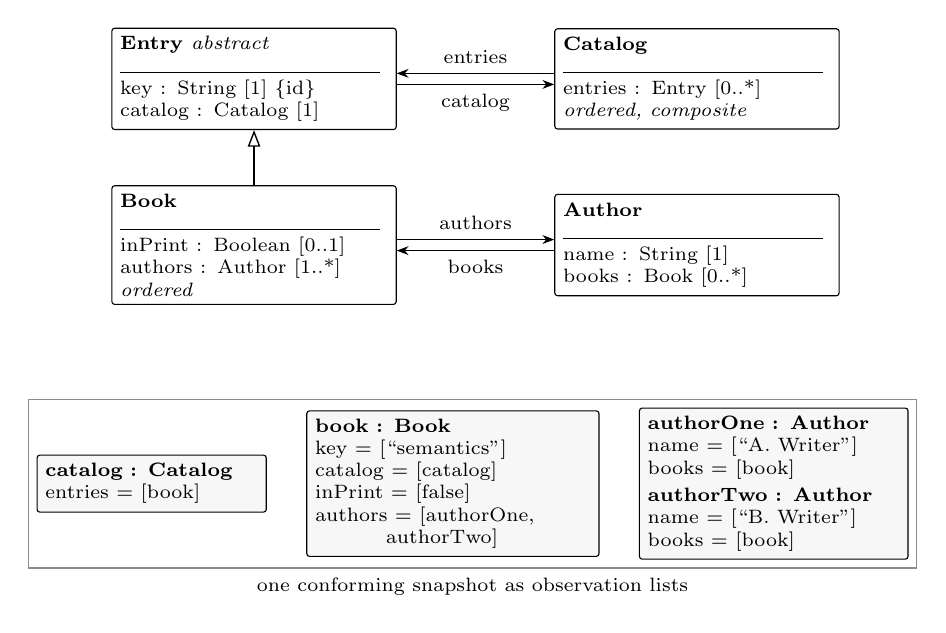
\begin{tikzpicture}[
  font=\scriptsize,
  cls/.style={draw,rounded corners=1pt,align=left,inner sep=3pt,text width=34mm},
  obj/.style={draw,rounded corners=1pt,align=left,inner sep=3pt,fill=black!3},
  rel/.style={-{Stealth[length=1.5mm]},line width=.45pt},
  note/.style={align=left,text width=30mm}
]
\node[cls] (entry) {\textbf{Entry} \emph{abstract}\\\rule{33mm}{.2pt}\\key : String [1] \{id\}\\catalog : Catalog [1]};
\node[cls,below=7mm of entry] (book) {\textbf{Book}\\\rule{33mm}{.2pt}\\inPrint : Boolean [0..1]\\authors : Author [1..*]\\\emph{ordered}};
\node[cls,right=20mm of book] (author) {\textbf{Author}\\\rule{33mm}{.2pt}\\name : String [1]\\books : Book [0..*]};
\node[cls,right=20mm of entry] (catalog) {\textbf{Catalog}\\\rule{33mm}{.2pt}\\entries : Entry [0..*]\\\emph{ordered, composite}};
\draw[-{Triangle[open,length=2.1mm]},line width=.5pt] (book) -- (entry);
\draw[rel] ([yshift=2pt]catalog.west) -- node[above,sloped]{entries} ([yshift=2pt]entry.east);
\draw[rel] ([yshift=-2pt]entry.east) -- node[below,sloped]{catalog} ([yshift=-2pt]catalog.west);
\draw[rel] ([yshift=2pt]book.east) -- node[above,sloped]{authors} ([yshift=2pt]author.west);
\draw[rel] ([yshift=-2pt]author.west) -- node[below,sloped]{books} ([yshift=-2pt]book.east);

\node[obj,below=19mm of book,xshift=-13mm,text width=27mm] (co)
  {\textbf{catalog : Catalog}\\entries = [book]};
\node[obj,right=5mm of co,text width=35mm] (bo)
  {\textbf{book : Book}\\key = [``semantics'']\\catalog = [catalog]\\inPrint = [false]\\authors = [authorOne,\\\hspace*{9mm}authorTwo]};
\node[obj,right=5mm of bo,text width=32mm] (au)
  {\textbf{authorOne : Author}\\name = [``A. Writer'']\\books = [book]\\[2pt]
   \textbf{authorTwo : Author}\\name = [``B. Writer'']\\books = [book]};
\node[draw=black!45,fit=(co)(bo)(au),inner sep=3pt,label={[font=\scriptsize]below:one conforming snapshot as observation lists}] {};
\end{tikzpicture}
\caption{Running catalog example. The lower panel exposes the actual observation
lists: paired rows record both association ends. The composite \emph{entries}
reference gives \emph{book} one incoming containment occurrence, and
\emph{key} applies to \emph{book} by inheritance. All properties are unique.}
\label{fig:catalog}
\end{figure}

Consider a catalog editor that adds a second author to a book. Updating only
\texttt{Book::authors} leaves both ends within their declared multiplicities:
the book has two authors and the new author's optional \texttt{books} list may
still be empty. Every value can also have the right type. Yet the resulting
snapshot is inconsistent: the two ends disagree about whether the authorship
exists. Checking each field in isolation cannot establish conformance.
Figure~\ref{fig:catalog} shows the completed update, with both ends recorded.

Several facts must agree even in this small example. The alias \texttt{Entry::key} denotes one declaration inherited by the
\emph{book} object. The list \texttt{Book::authors} records two ordered object
identities. Each occurrence must be matched at the opposite end by a
\texttt{Author::books} occurrence. The book is contained once through
\texttt{Catalog::entries}, while the upper-one \texttt{Entry::catalog} end
records the inverse. These are related parts of one conformance judgment, not
independent validation options.

The source also records \texttt{Book::inPrint = [false]}. Because the property is
optional, \texttt{[]} would also satisfy its multiplicity, but it would describe
absence rather than the Boolean value false. This distinction matters when the
same model is realized in a format with default-value behavior.

The central source fragment is readable without exposing allocated identifiers:

\noindent\begin{minipage}{\linewidth}
\begin{verbatim}
object book : Book {
  observe Entry::key = ["semantics"];
  observe Entry::catalog = [@catalog];
  observe Book::inPrint = [false];
  observe Book::authors = [@authorOne, @authorTwo];
}
\end{verbatim}
\end{minipage}

The complete listing in the artifact includes the catalog, authors, both
associations, and every required observation; the current command-line checker
accepts it. The modeling question is whether this acceptance has the same
meaning as the symbolic document. Answering it requires both a precise account
of finite EMOF conformance and a proof about the elaboration that replaces
aliases with identities.

\section{Formalization}\label{sec:formalization}
\subsection{Representation}\label{sec:representation}
We write $\langle x_1,\ldots,x_n\rangle$ for a finite sequence and $\langle\rangle$
for the empty one; $|L|$ is the length of a sequence $L$, and $\#_v(L)$ the number
of occurrences of $v$ in it.

\begin{definition}[Schema]\label{def:schema}
A \emph{schema} $S$ consists of finite lists of declarations, each with an
identity and a simple name, that refer to each other by identity:
\begin{list}{}{\setlength{\leftmargin}{6mm}\setlength{\labelwidth}{5mm}%
 \setlength{\itemsep}{0pt}\setlength{\parsep}{0pt}\setlength{\topsep}{1pt}}
\item[(a)] packages, each with an optional parent package;
\item[(b)] classes, each with a package, direct superclasses and an abstract flag;
\item[(c)] properties $p$, each with an owner (a class or an association), a type
 (Boolean, integer, string, an enumeration or a class), bounds
 $\ell_p\in\mathbb N$ and $u_p\in\mathbb N\cup\{\ast\}$, where $\ast$ is
 unbounded, and flags $\mathit{unique}_p$, $\mathit{composite}_p$ and
 $\mathit{id}_p$ (identifier);
\item[(d)] associations, each with a package and two \emph{opposite ends} $(p,q)$;
\item[(e)] enumerations, each with a package, and literals, each with its enumeration.
\end{list}
\end{definition}

\begin{definition}[Snapshot]\label{def:snapshot}
A \emph{snapshot} $M=(O,\mathit{cls},R)$ consists of a finite list $O$ of object
identities, each with a class identity $\mathit{cls}(o)$, and a finite list $R$
of \emph{observation rows} $(o,p,L)$: an object identity, a property identity and
a sequence $L$ of values. A value is an object reference $\operatorname{ref}(o)$,
a Boolean, an integer, a string or an enumeration literal. We call $(S,M)$ a
\emph{Core} pair.
\end{definition}

\begin{definition}[Lookup]\label{def:lookup}
Let $(o,p,L_1),\ldots,(o,p,L_k)$ be the rows of $R$ for object $o$ and
property $p$, in their order in $R$. The \emph{lookup} of $p$ on $o$ is their
concatenation
\[
 L_M(o,p)=L_1L_2\cdots L_k,
\]
which is $\langle\rangle$ if $k=0$. We write $o.p$ for $L_M(o,p)$.
\end{definition}

\paragraph{Applicability.}
The \emph{ancestors} of a class are the class itself and the classes reached
through direct superclasses. A property $p$ \emph{applies} to class $c$, written
$p\in\mathit{app}(c)$, if an ancestor of $c$ declares $p$, or if $p$ is an
association-owned end whose opposite has an ancestor of $c$ as its type.
Following UML inheritance and EMOF property access
\cite{omg_uml_25,omg_mof_251}, inherited properties are collected by
declaration identity: a diamond yields one declaration, and same-named ones are
selected by qualified names, not overridden; e.g., \emph{RailwayElement.id}
applies to \emph{Switch}.

Figure~\ref{fig:running} shows our running snapshot $M_T$ as a UML object
diagram over the metamodel of Figure~\ref{fig:train}: route $r$ requires sensors
$s_A,s_B$ and follows switch position $\mathit{sp}$ of switch $\mathit{sw}$.
Each slot and each link end is one row. The two \emph{requires} links form the
single row $(r,\mathit{requires},\langle\operatorname{ref}(s_A),\operatorname{ref}(s_B)\rangle)$,
and the link between $r$ and $\mathit{sp}$ gives
$r.\mathit{follows}=\langle\operatorname{ref}(\mathit{sp})\rangle$ and
$\mathit{sp}.\mathit{route}=\langle\operatorname{ref}(r)\rangle$. Every other
applicable property, such as $r.\mathit{entry}$, has an empty row.

\begin{figure}[!t]
\centering
\def\objbox#1#2{\begin{tabular}{@{\hspace{3pt}}l@{\hspace{3pt}}}\underline{#1}\\[1.5pt]\hline #2\end{tabular}}
\resizebox{.8\linewidth}{!}{%
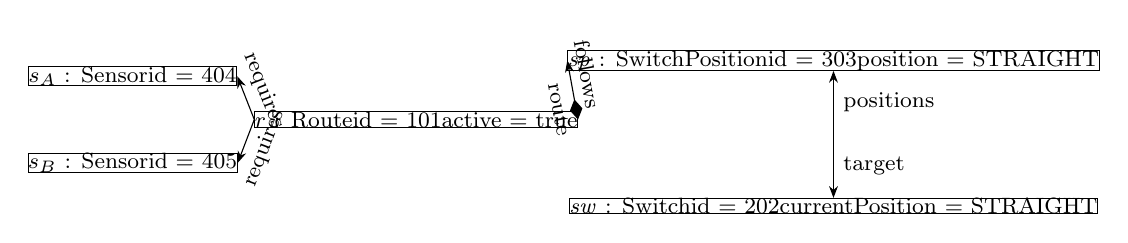
\begin{tikzpicture}[font=\footnotesize,
 obj/.style={draw,inner sep=0pt},
 nav/.style={-{Stealth[length=1.5mm]}},
 comp/.style={{Diamond[length=2.6mm,width=1.6mm]}-{Stealth[length=1.5mm]}},
 both/.style={{Stealth[length=1.5mm]}-{Stealth[length=1.5mm]}}]
\node[obj] (sA) at (0.4,0.65) {\objbox{$s_A$ : Sensor}{id = 404}};
\node[obj] (sB) at (0.4,-0.45) {\objbox{$s_B$ : Sensor}{id = 405}};
\node[obj] (r) at (4.0,0.1) {\objbox{$r$ : Route}{id = 101\\ active = true}};
\node[obj] (sp) at (9.3,0.85) {\objbox{$\mathit{sp}$ : SwitchPosition}{id = 303\\ position = STRAIGHT}};
\node[obj] (sw) at (9.3,-1.0) {\objbox{$\mathit{sw}$ : Switch}{id = 202\\ currentPosition = STRAIGHT}};
\draw[nav] (r.west) -- node[pos=.5,above,sloped]{requires} (sA.east);
\draw[nav] (r.west) -- node[pos=.5,below,sloped]{requires} (sB.east);
\draw[comp] (r.east) -- node[pos=.22,below,sloped]{route} node[pos=.72,above,sloped]{follows} (sp.west);
\draw[both] (sp.south) -- node[pos=.25,right]{positions} node[pos=.75,right]{target} (sw.north);
\end{tikzpicture}}
\caption{Running snapshot $M_T$ of the metamodel in Figure~\ref{fig:train}.}
\label{fig:running}
\end{figure}

With one row per pair, as in $M_T$, lookup returns that row's sequence, and an
empty row records absence: $r.\mathit{entry}=\langle\rangle$ differs from
$\langle\mathsf{false}\rangle$ or $\langle 0\rangle$. Lookup is also defined for
a missing row, giving $\langle\rangle$, and for repeated rows, which concatenate.

\subsection{Structural Conformance}\label{sec:conformance}
Definitions~\ref{def:wellformed} and~\ref{def:conformance} adapt structural
clauses of UML and MOF, as argued from their text and an audit of MOF~\S12.4's
32 EMOF restrictions. Below, we trace the conditions to the original
specifications and demonstrate them with counterexamples, i.e., variants of $M_T$
that each violate a single condition.

\begin{definition}[Well-formedness]\label{def:wellformed}
A schema $S$ is \emph{well formed}, $W(S)$, if:
\begin{list}{}{\setlength{\leftmargin}{9mm}\setlength{\labelwidth}{8mm}%
 \setlength{\itemsep}{1pt}\setlength{\parsep}{0pt}\setlength{\topsep}{2pt}}
\item[(W1)] \emph{Identities}: declarations of each kind have distinct identities.
\item[(W2)] \emph{Names}: every name is nonempty and consists of XML-valid characters.
\item[(W3)] \emph{Resolution}: every reference between declarations resolves to
 one of the expected kind, and an association owning a property has it as an end.
\item[(W4)] \emph{Acyclicity}: package nesting and generalization are acyclic.
\item[(W5)] \emph{Properties}: $\ell_p\leq u_p$; composite properties have class
 types; and a class has at most one identifier, declared or inherited.
\item[(W6)] \emph{Associations}: the two ends are distinct and class-typed, at
 most one is association-owned, and a class-owned end is owned by the type of its
 opposite; no property is an end of two associations; and the opposite of a composite
 end is not composite and has upper bound~1.
\end{list}
\end{definition}
W2, W5 and W6 include EMOF restrictions \cite{omg_mof_251}; W4 and the composite
conditions follow UML \cite{omg_uml_25}.

\begin{definition}[Conformance]\label{def:conformance}
A snapshot $M$ \emph{conforms} to a schema $S$, written $C(S,M)$, if $W(S)$
holds and, for all $o\in O$ and $p\in\mathit{app}(\mathit{cls}(o))$:
\begin{list}{}{\setlength{\leftmargin}{9mm}\setlength{\labelwidth}{8mm}%
 \setlength{\itemsep}{1pt}\setlength{\parsep}{0pt}\setlength{\topsep}{2pt}}
\item[(C1)] \emph{Objects}: identities are distinct, and $\mathit{cls}(o)$ is
 resolved and not abstract.
\item[(C2)] \emph{Rows}: every row names a stored object and a property that
 applies to its class, and the pair $(o,p)$ has exactly one row.
\item[(C3)] \emph{Typing}: every value in $L_M(o,p)$ fits the type of $p$:
 references to stored objects whose class has that type as an ancestor, literals
 of the enumeration, or XML-valid strings.
\item[(C4)] \emph{Multiplicity}: $\ell_p\leq|L_M(o,p)|\leq u_p$, and if
 $\mathit{unique}_p$, no value repeats in $L_M(o,p)$.
\item[(C5)] \emph{Opposites}: for each association $(p,q)$ and all $x,y\in O$,
 $\#_{\operatorname{ref}(y)}L_M(x,p)=\#_{\operatorname{ref}(x)}L_M(y,q)$.
\item[(C6)] \emph{Containment}: $o$ has at most one \emph{parent}, i.e., an
 $x\in O$ with $\operatorname{ref}(o)\in L_M(x,p')$ for a composite $p'$; at most
 one \emph{container end} $q$ of $o$, the opposite of a composite property, has
 $L_M(o,q)\neq\langle\rangle$; and no chain of parents leads from an object back
 to itself.
\end{list}
\end{definition}

\paragraph{Objects, rows and typing (C1--C3).}
C1 follows UML: abstract classes have no direct instances \cite{omg_uml_25}.
C2 demands the rows of Section~\ref{sec:representation}, recording MOF's null
or empty list \cite{omg_mof_251} as $\langle\rangle$, so it rejects missing and
repeated rows; deleting $\mathit{sw}$'s \emph{id} row violates it alone. C3
follows UML type conformance and MOF's XML Schema datatypes.

\paragraph{Multiplicity (C4).}
Following UML \cite{omg_uml_25}, bounds count occurrences, and uniqueness
separately excludes repeats. Dropping $s_B$ from $M_T$ leaves
$|r.\mathit{requires}|=1<2$, which violates C4 alone. A $0..0$ bound means that
a property stays empty; MOF requires positive upper bounds only before
reflective \texttt{create} \cite[\S9.3.3]{omg_mof_251}, which our subset omits.

\paragraph{Opposites (C5).}
Without link identities, an association is observed at both ends, and C5 makes
the ends agree occurrence by occurrence. Clearing $\mathit{sp}.\mathit{route}$
in $M_T$ gives $0\neq1$ against $r.\mathit{follows}$: a link recorded at one end
only. For unique ends, C5 is reciprocal membership; with mixed uniqueness, it is
stricter than UML \cite[\S11.5.3.1]{omg_uml_25}. Were the unique
\emph{Route.follows} nonunique, UML would permit two links between $r$ and
$\mathit{sp}$, seen as
$\langle\operatorname{ref}(\mathit{sp}),\operatorname{ref}(\mathit{sp})\rangle$
at \emph{follows} but $\langle\operatorname{ref}(r)\rangle$ at the unique
\emph{route} end; C5 rejects this ($2\neq1$), a restriction of our subset.

\paragraph{Containment (C6).}
C6 follows MOF \cite[\S12.5.5]{omg_mof_251}. Parents form a set, so repeated
occurrences add none: a region listing
$\langle\operatorname{ref}(\mathit{seg}),\operatorname{ref}(\mathit{seg})\rangle$
gives $\mathit{seg}$ one parent. Only the uniqueness of \emph{Region.elements}
(C4) rejects this list; with uniqueness disabled, it is accepted. A segment in the
\emph{elements} of two regions violates C6 alone.

\subsection{Verified Checking and Translation}\label{sec:guarantees}
We prove that the checker accepts exactly the conforming pairs and that
elaboration preserves meaning; Section~\ref{sec:tool} describes the Lean
mechanization.

\begin{theorem}[Checker correctness]\label{thm:checker}
For every schema $S$ and snapshot $M$, the checker's Boolean verdict satisfies
\begin{equation}
 \operatorname{check}(S,M)=\mathsf{true}
 \quad\Longleftrightarrow\quad C(S,M).
\label{eq:checker}
\end{equation}
\end{theorem}
\begin{proofsketch}
Apart from reachability, each condition of Definitions~\ref{def:wellformed}
and~\ref{def:conformance} quantifies over the finite lists of $S$ and $M$, e.g.,
C4 over $O$ and $\mathit{app}(\mathit{cls}(o))$, and the checker evaluates it
element by element, which is exact. For the ancestors of a class $c$, it
computes, as breadth-first search does, $X_0=\{c\}$ and
$X_{k+1}=X_k\cup\mathit{sup}(X_k)$, where $\mathit{sup}(X)$ holds the direct
superclasses of the classes in $X$; for \emph{Switch}, $X_1$ adds
\emph{TrackElement}, $X_2$ adds \emph{RailwayElement}, and $X_3=X_2$. Under W3,
$X_0\subseteq X_1\subseteq\cdots$ lie among the $n$ classes of $S$, so $X_{n+1}=X_n$:
$X_n$ is closed under $\mathit{sup}$, hence contains every ancestor, and it
contains only ancestors. Package nesting (W4) and parent chains (C6) are alike;
there, W3, C2 and C3 keep links within the lists. A pair violating these does not conform and is rejected, as the
checker evaluates them too.
\end{proofsketch}

\paragraph{From source documents to Core.}
Theorem~\ref{thm:checker} concerns Core pairs, but users write text, which a
parser turns into a source document that uses names instead of identities.
Translating it into Core must preserve its meaning: dropping a repeated value
would hide a uniqueness violation (C4), and merging two names would create one.
We therefore define the translation and, independently of it, what a source
document means.

\begin{definition}[Source document]\label{def:document}
A \emph{source document} $d$ has the components of Definitions~\ref{def:schema}
and~\ref{def:snapshot}, with names in place of identities: each declaration has
a \emph{qualified name}, a sequence of strings such as
$\mathit{Route}{::}\mathit{requires}$, besides its simple name; each object has an
\emph{object name}, such as $r$; and references and rows use these names. $L_d$ is
the lookup of $d$. We call $d$ \emph{well named}, i.e., its names can serve as identities, if:
\begin{list}{}{\setlength{\leftmargin}{9mm}\setlength{\labelwidth}{8mm}%
 \setlength{\itemsep}{1pt}\setlength{\parsep}{0pt}\setlength{\topsep}{2pt}}
\item[(N1)] every qualified and object name is nonempty and has nonempty components;
\item[(N2)] no two declarations, and no two objects, have the same name;
\item[(N3)] each declaration's qualified name extends its owner's by one
 component, or has one component if the declaration has no owner;
\item[(N4)] every name used in $d$ denotes a declaration or object of the expected kind.
\end{list}
We call $d$ \emph{lexically admissible} if the components of its qualified and
object names consist of XML-valid characters.
\end{definition}

\begin{definition}[Elaboration]\label{def:elaboration}
\emph{Elaboration} $E$ translates a source document $d$ into a Core pair. It fails
unless $d$ is well named; otherwise $E(d)=\mathsf{ok}(\rho(d))$. Here $\rho$
numbers the declarations of each kind and the objects by their positions in $d$,
and $\rho(d)$ replaces every qualified or object name $n$ by $\rho(n)$, keeping
simple names and the order and repetition of values.
\end{definition}
Elaborating the source document of $M_T$, whose objects are named $r$, $s_A$,
$s_B$, $\mathit{sp}$ and $\mathit{sw}$, yields $M_T$ up to the choice of
identities; naming two objects $r$ makes elaboration fail by (N2).

\begin{definition}[Source meaning]\label{def:meaning}
The \emph{meaning} of a source document $d$ is the condition $\mathcal S(d)$ that
$d$ is well named and lexically admissible and that $W$ and C1--C6 hold on $d$
with names in place of identities.
\end{definition}
$\mathcal S(d)$ is stated on $d$ alone, without $E$ or $\rho$. Elaboration checks every name condition of $\mathcal S(d)$ except lexical
admissibility, which a Core pair cannot confirm, since it keeps no qualified or
object names.

\begin{theorem}[Elaboration adequacy]\label{thm:adequacy}
Let $d$ be a lexically admissible source document. (i)~If $\mathcal S(d)$, then
$E(d)$ succeeds. (ii)~If $E(d)=\mathsf{ok}(S,M)$, then $\mathcal S(d)\Leftrightarrow C(S,M)$.
\end{theorem}
Part~(i) says that elaboration rejects only documents whose meaning fails, and
part~(ii) that a successful elaboration neither hides nor introduces violations.
\begin{proofsketch}
(i)~Elaboration fails only if $d$ is not well named, which $\mathcal S(d)$ rules
out. (ii)~By (N2), $\rho$ is a bijection from the names of $d$ onto the identities of
$E(d)=\rho(d)$, which keeps every row and the order and repetition of its
values; hence $L_{E(d)}(\rho o,\rho p)=\rho(L_d(o,p))$, and $\rho$ is an
isomorphism from $d$ onto $E(d)$. $W$ and C1--C6 refer to identities only
through equality, lookup and references, which isomorphisms preserve, so each
holds on $d$ exactly when it holds on $E(d)$. The faulty translations above are
not isomorphisms: dropping a repeat changes a lookup, and merging two names
breaks injectivity. For $C(S,M)\Rightarrow\mathcal S(d)$, only the name conditions
remain: $d$ is well named because $E(d)$ succeeded, and lexically admissible by
hypothesis.
\end{proofsketch}
With Theorem~\ref{thm:checker}, every lexically admissible source document $d$
with $E(d)=\mathsf{ok}(S,M)$ thus satisfies
\begin{equation}
 \mathcal S(d)
 \ \overset{\text{Thm.~\ref{thm:adequacy}}}{\Longleftrightarrow}\
 C(S,M)
 \ \overset{\text{Thm.~\ref{thm:checker}}}{\Longleftrightarrow}\
 \operatorname{check}(S,M)=\mathsf{true},
\label{eq:adequacy}
\end{equation}
and by~(i), $\mathcal S(d)$ fails whenever $E(d)$ fails. Checking the elaborated
pair thus answers exactly whether a source document satisfies its meaning.

\section{Tool Support}
\subsection{One checker, three input routes}
The command-line tool accepts symbolic text and versioned Core JSON. Both reach
the same checker; reports distinguish conformance failures, binding/decoding
errors and unsupported inputs. Figure~\ref{fig:boundary} locates the proved
connections. Equation~\ref{eq:adequacy} begins at the AST, outside the parser.
The JSON decoder admits malformed represented records for the checker to reject;
its key-normalization policy is documented separately.

\begin{figure}[t]
\centering
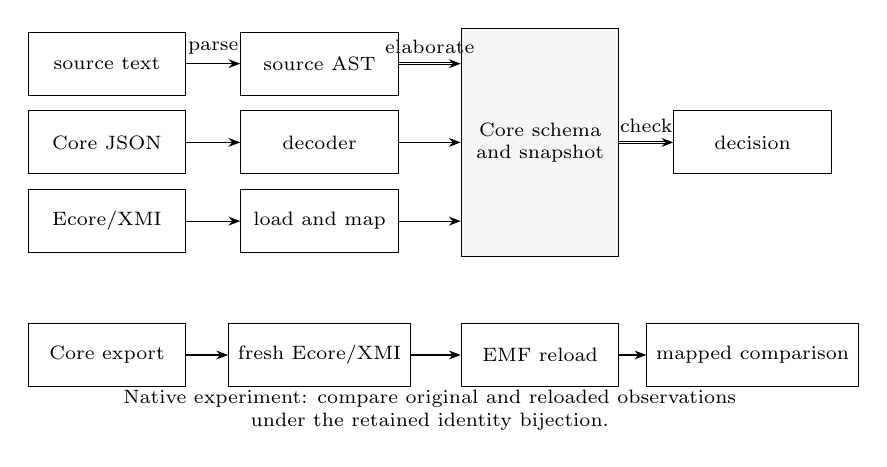
\begin{tikzpicture}[font=\scriptsize,
 box/.style={draw,align=center,minimum width=20mm,minimum height=8mm},
 arr/.style={-{Stealth[length=1.5mm]}}]
\node[box] (text) at (-4,1) {source text};
\node[box] (ast) at (-1.3,1) {source AST};
\node[box] (json) at (-4,0) {Core JSON};
\node[box] (decode) at (-1.3,0) {decoder};
\node[box] (native) at (-4,-1) {Ecore/XMI};
\node[box] (map) at (-1.3,-1) {load and map};
\node[box,minimum height=29mm,fill=black!4] (core) at (1.5,0) {Core schema\\and snapshot};
\node[box] (check) at (4.2,0) {decision};
\draw[arr] (text) -- node[above]{parse} (ast);
\draw[arr,double,double distance=.5pt] (ast) -- node[above]{elaborate} ([yshift=10mm]core.west);
\draw[arr] (json) -- (decode);
\draw[arr] (decode) -- (core);
\draw[arr] (native) -- (map);
\draw[arr] (map) -- ([yshift=-10mm]core.west);
\draw[arr,double,double distance=.5pt] (core) -- node[above]{check} (check);
\node[box] (export) at (-4,-2.7) {Core export};
\node[box] (fresh) at (-1.3,-2.7) {fresh Ecore/XMI};
\node[box] (reload) at (1.5,-2.7) {EMF reload};
\node[box] (compare) at (4.2,-2.7) {mapped comparison};
\draw[arr] (export) -- (fresh);
\draw[arr] (fresh) -- (reload);
\draw[arr] (reload) -- (compare);
\node[align=center] at (.1,-3.4) {Native experiment: compare original and reloaded observations\\under the retained identity bijection.};
\end{tikzpicture}
\caption{Input routes and the separate native round-trip experiment. Double
arrows identify computations covered by formal correspondence results under
their stated premises. Parsing, codecs, loading and native comparison are tested
boundaries. An actual EMF validator is a separate experimental oracle.}
\label{fig:boundary}
\end{figure}

\subsection{Restricted EMF realization}
The Java bridge loads Ecore/XMI through dynamic EMF objects. Its restricted
profile rejects unsupported annotations, operations, generics, declared defaults,
derived/unsettable features, custom datatypes and unresolved references. Export
also requires class-owned association ends, representable packages/names and
signed 32-bit integers.

Import allocates identities from containment. An XML pass tracks written scalar
values separately from omitted ones. This lexical policy can differ from native
\texttt{eIsSet}, especially for enumeration defaults; Section~5 reports an actual
mismatch. Lossless alignment is therefore checked per input, not assumed from
successful import.

Export constructs fresh resources, establishes both opposite pointers and compares
observations before serialization. A sidecar maps Core identities to native URIs.
Reload comparison requires a bijection, remaps references, and compares sequences
or multisets according to ordering. These are executable checks outside the Lean
proof, not universal codec correctness results.

\subsection{Reuse for bounded metadata}
A fixed metadata vocabulary represents class and scalar-attribute descriptions
as ordinary objects and properties. The common checker validates a description
before an interpreter produces a Core schema. The example describes an optional
Boolean property and then checks an instance of the resulting class. A dangling
owner is rejected as metadata; reversed bounds can be well-typed metadata yet
produce an invalid interpreted schema. This separates validity of the
description graph from validity of what it denotes.

\section{Evaluation}\label{sec:evaluation}
\subsection{Cases and Semantic Checks}
We combine public inputs with models constructed for this study. From the
Train v1.0 repository\footnote{\url{https://github.com/FTSRG/trainbenchmark/tree/v1.0}}
\cite{szarnyas_etal_2018}, we take its railway metamodel and first stored batch
snapshot, a generated benchmark model rather than operational railway data.
After adapting the metamodel to the supported Ecore subset, we import the
unchanged snapshot: ten classes, 21 features, two enumerations, 754 objects and
3,378 observation rows. Our generated textual rendition elaborates exactly to
that Core pair, including identities, flags, row order and absence. Removing all
but one required sensor from a Route gives a multiplicity failure while the
other structural checks pass.

We construct the other positive and negative cases to isolate typing,
multiplicity, inheritance, opposites and containment. The nine scaling inputs
in Section~\ref{sec:timing} and two small authored examples form the eleven
aligned positives in Table~\ref{tab:correctness}; they are not eleven independent
metamodels. An additional public input, the EMF Compare metamodel from its
3.3.28 repository, is rejected by the bridge for unsupported operations before
Core checking. The input and runner index is \texttt{experiments/README.md};
public originals are acquired separately, and historical measurement logs are
kept outside the source repository. The artifact records revisions, adaptations
and licenses.

For RQ1, Section~\ref{sec:conformance} supplies the source correspondence and
subset restrictions; these cases illustrate consequences of the predicates.
Section~\ref{sec:guarantees}'s proofs address RQ2. A Lean proof client derives
nonconformance from a repeated link with an upper-one opposite, exercising
Proposition~\ref{prop:opposite} under our equal-count restriction.

\subsection{Comparison with EMF}
We use EMF Ecore/XMI 2.39.0 and Common 2.42.0 under Java~21. An isolated registry selects EcoreValidator and generic
EObjectValidator for dynamic instances; Diagnostician checks schema and instance
roots separately. Generated validators and OCL delegates are excluded.
Table~\ref{tab:correctness}(a) separates these calls from VL-MOF's combined check:
instance acceptance cannot override schema rejection. Panel (b) reports the loaded-model comparison of Section~\ref{sec:tool}.
It uses values when native \texttt{eIsSet} holds and an empty sequence otherwise,
not unconditional \texttt{eGet}; equal states can still receive different decisions.
These comparisons measure agreement under the stated configurations; they do
not establish either validator's fidelity to EMOF.

\begin{table}[tbp]
\centering\small
\caption{Validation decisions (a) and loaded-state correspondence (b).}
\label{tab:correctness}
\textbf{(a) Validation decisions}\\[3pt]
\begin{tabular}{p{49mm}ccc}
\hline
Case & EMF schema & EMF instance & VL-MOF \\
\hline
Aligned positives (11) & Accept & Accept & Accept \\
Missing required String & Accept & Reject & Reject \\
Repeated unique String & Accept & Accept & Reject \\
Train with explicit defaults & Accept & Accept & Accept \\
Train with original omissions & Accept & Accept & Accept \\
\hline
Lower 1 / upper 0 & Reject & Reject & Reject \\
Empty $0..0$ & Reject & Accept & Accept \\
Repeated containment & Reject & Accept & Accept \\
Two unpaired features & Reject & Accept & Accept \\
\hline
\end{tabular}

\medskip
\textbf{(b) Correspondence after loading}\\[3pt]
\begin{tabular}{>{\raggedright\arraybackslash}p{54mm}>{\raggedright\arraybackslash}p{60mm}}
\hline
Case(s) & State comparison \\
\hline
All cases in (a) except those below & Match \\
Train with explicit defaults & 12 scalar-presence differences \\
Repeated containment; two unpaired features & Comparison fails: duplicate collector rows from repeated visits \\
\hline
\end{tabular}
\end{table}

The lower block of Table~\ref{tab:correctness}(a) exposes Ecore schema
restrictions. In particular, an empty $0..0$ property is permitted by our
structural interpretation but rejected by Ecore at schema level.
The repeated unique String survives loading but is accepted by this generic
validator and rejected by VL-MOF; it does not establish the behavior of every
EMF editor or generated validator. Repeated traversal of a contained object
produces duplicate collector rows in the two unpaired cases. Their alignment is
conservatively unsuccessful even though their distinct URI/value comparisons
agree; they are not timed. The two-feature fixture shares a schema containing
an additional nonunique composite \emph{children} declaration. Its schema
rejection therefore does not isolate the two-feature instance behavior.

Our adaptation of the Train v1.0 metamodel removes one generator annotation and maps EJavaObject
attributes to EInt (\emph{id}, \emph{length}) and EBoolean (\emph{active}). It uses
$0..1$ for \emph{route}, \emph{target}, \emph{entry} and \emph{exit}, versus one in
the article's diagram; Figure~\ref{fig:train} shows the evaluated metamodel.
We also create a copy of the public snapshot with omitted enum defaults
written explicitly. In this default-materialized copy, native
\texttt{eIsSet} reports twelve explicit first-enumeration values unset while
bridge import retains \texttt{FAILURE}. Both validators accept, despite singleton
versus empty observations. This case is excluded from paired timing. The original-snapshot control
with adapted Ecore instead aligns and is accepted by
both: zero lower bounds permit omissions without inserting defaults. This result
is specific to the adapted metamodel; the unadapted schema is unsupported.

\subsection{Validation Time}\label{sec:timing}
We generate three workload families ourselves to vary size and shape while
holding each family's schema fixed. A \emph{containment star} has one parent
and many children with inherited scalar features and ordered value lists
(11/101/501 objects). A \emph{Train projection} repeats our five-object
route/switch example, with optional bounds (2/20/100 groups). A
\emph{containment chain} nests each child inside its predecessor
(11/101/501 objects, depths 10/100/500). These are synthetic tests of our checker,
not executions of the Train Benchmark's query workload; the public 754-object
snapshot is not timed. The artifact records structural counts; a chain of $N$ objects has $3N-2$ value occurrences.

Each case uses five independent process trials, ten warmups and thirty measured
repetitions, with both tool orders and alternate traversal directions. Builds
precede timing. We measure combined schema/instance validation on preloaded
inputs, excluding loading, serialization and diagnostics. The artifact also
records VL-MOF schema-only and read/decode phases, plus command-wall times;
EMF schema-only and load/decode phases were not retained. Instance-only validation
was not measured and cannot be inferred by subtracting schema time.

Table~\ref{tab:validation-times} reports the median of five process medians
in milliseconds; the artifact retains each process median, their minimum and
maximum, and all measured samples. Rows count feature observations.
\begin{table}[t]
\centering
\caption{Preloaded combined schema--instance validation time in ms: pooled
median [first, third quartile] from five independent processes, each with 10 warmups and 30
retained samples. Rows are complete feature-observation rows.}
\label{tab:validation-times}
\scriptsize
\setlength{\tabcolsep}{3pt}
\begin{tabular}{lrrll}
\hline
Family/shape & Objects & Rows & EMF & VL-MOF \\
\hline
Containment star & 11  & 42   & 0.654 [0.452, 0.950] & 0.677 [0.664, 0.712] \\
Containment star & 101 & 402  & 0.725 [0.533, 0.956] & 9.664 [9.477, 9.974] \\
Containment star & 501 & 2002 & 1.582 [1.152, 2.116] & 125.713 [123.854, 127.518] \\
Train projection & 10  & 26   & 0.768 [0.464, 1.121] & 2.231 [2.194, 2.287] \\
Train projection & 100 & 260  & 0.944 [0.756, 1.257] & 24.840 [24.353, 25.412] \\
Train projection & 500 & 1300 & 1.726 [1.270, 2.362] & 169.457 [158.682, 171.603] \\
Containment chain & 11  & 33   & 0.515 [0.381, 0.723] & 0.154 [0.152, 0.164] \\
Containment chain & 101 & 303  & 0.828 [0.600, 1.056] & 109.293 [107.933, 111.918] \\
Containment chain & 501 & 1503 & 2.037 [1.556, 2.834] & timeout \\
\hline
\end{tabular}
\end{table}

Each completed cell contains 150 samples per tool. For the 501-object chain,
all five EMF processes completed and supply the reported 150 samples. Each
VL-MOF benchmark process exceeded its 120-second process limit before emitting
its buffered sample array, so there are no retained VL-MOF samples for that
cell. This bounds the whole 40-iteration benchmark process; it does not show
that one validation takes 120 seconds.

The results show sensitivity to graph shape as well as size. At 101 objects,
VL-MOF's chain median is about eleven times its star median, although the chain
has fewer observation rows. EMF remains below 3 ms at the pooled median for
these inputs. These descriptive measurements compare the current implementations,
whose data structures and runtimes differ; they are neither an asymptotic result
nor evidence of a general speed ranking. Loading, parsing, normalization,
diagnostics, and process startup lie outside the measured window.


For RQ3, 40 of 45 paired timing trials complete; five VL-MOF processes time out
on the deepest chain. Raw samples and excluded preliminary runs remain in the artifact.

\section{Discussion}
\subsection{Related Work}
\paragraph{Formal conformance and MOF semantics.}
Paige et al. formalize metamodel conformance and multiview consistency in PVS
and Eiffel, distinguishing mathematical analysis from confidence that the
formal specification captures the intended metamodel
\cite{paige_brooke_ostroff_2007}.

Boronat and Meseguer give executable MOF semantics using membership-equational
theories \cite{boronat_meseguer_2010}. Their work formalizes models, metamodels
and conformance, including sets, ordered sets, bags and sequences. Executable conformance and these collection semantics are established precedents. Their detailed EMOF/OCL account restricts structural lower bounds
to zero or one and upper bounds to one or unlimited; it also assumes that every
composite property has an opposite \cite{boronat_meseguer_report}. VL-MOF admits
general finite bounds and unpaired composite properties. These are differences
from the stated structural profile, not a claim that additional constraints
cannot be expressed in the earlier framework.

Our contribution lies in the connection between a documented EMOF~2.5.1
interpretation and two mechanized guarantees: checker equivalence for arbitrary
represented inputs, and correspondence between independently defined symbolic
satisfaction and elaboration. Coverage equivalence or greater expressiveness would require a translation
between the formalisms, which we do not establish.

\paragraph{Containment and model changes.}
K\"ohler et al. constrain incoming containment edges and cycles in instance
graphs and derive preservation conditions for graph transformations
\cite{koehler_lewin_taentzer_2007}. VL-MOF distinguishes repeated occurrences
of a link from distinct parent identities, and checks active reverse container
properties separately. This choice matters for nonunique composite features.
Coq4MDE proves preservation for ISC model composition, with injectivity and
freshness conditions relevant to multiplicities \cite{kezadri_etal_2014}.
Its opposite condition compares membership, whereas ours compares occurrence
counts.

\paragraph{Textual metamodeling.}
NEREUS and KM3 provide formal and textual approaches to metamodel specification,
while Emfatic and Xcore support textual Ecore definitions
\cite{favre_duarte_2016,jouault_bezivin_2006,emfatic_docs,xcore_docs}.
VL-MOF uses named declarations to expose its semantics, with a proved link
from their independent meaning to Core conformance.

\subsection{Threats to Validity}
\paragraph{Construct validity.}
A correct checker can implement an unsuitable interpretation of EMOF. We address
this risk through clause-level traceability and examples that separate competing
interpretations; neither replaces a proof of fidelity to the standard's prose.
The representation also assumes complete finite snapshots with an implicit
outer scope. Its conclusions therefore apply to that structural setting, with
the Train profile adaptations stated in Section~5.2.

\paragraph{Internal validity.}
The proofs begin at the AST or Core boundary. Errors in parsing, JSON conversion,
the Java bridge or the measurement harness can affect an end-to-end result.
Exact Train reconstruction and loaded-state comparisons test these boundaries
on the selected inputs. They provide evidence about those cases, not general
correctness of interchange, inverse maintenance or default/unset behavior.
Historical generation and orchestration sources were not hashed. Retained
inputs, commands and raw samples support recomputing the reported summaries,
but cannot establish complete reproduction of the historical build.

\paragraph{External and conclusion validity.}
Train is the only public positive model family; the unchanged EMF Compare input
is outside the bridge profile. Synthetic sizes and shapes expose sensitivity
to model structure but do not establish industrial scalability. The EMF results
apply to the stated generic validator setup, not every editor or generated
validator. Timing summaries use independent process trials and retain their
ranges and timeouts in the artifact. They describe the measured workloads and
implementations, without isolating a bottleneck or establishing complexity bounds.

\section{Conclusion}
VL-MOF connects a source-audited structural EMOF interpretation to a proved
finite checker and conditional symbolic correspondence. The opposite-count
consequence rules out repeated-link edits across candidate snapshots without
assuming forward uniqueness. Native comparisons demonstrate why acceptance and
loaded-state alignment must remain separate; scaling exposes practical limits
of the present implementation.

Further work has concrete dependencies: reflective operations need transition
and preservation results; defaults/unset history need richer observation states;
full metadata interpretation needs packages, inheritance, references and
materialized ownership. The delivered static definitions and proofs support
that work without establishing those additional capabilities.

\bibliographystyle{splncs04}
\bibliography{references}
\end{document}
